%Header
    \documentclass[11pt]{article}\usepackage[]{graphicx}\usepackage[]{color}
%% maxwidth is the original width if it is less than linewidth
%% otherwise use linewidth (to make sure the graphics do not exceed the margin)
\makeatletter
\def\maxwidth{ %
  \ifdim\Gin@nat@width>\linewidth
    \linewidth
  \else
    \Gin@nat@width
  \fi
}
\makeatother

\definecolor{fgcolor}{rgb}{0.345, 0.345, 0.345}
\newcommand{\hlnum}[1]{\textcolor[rgb]{0.686,0.059,0.569}{#1}}%
\newcommand{\hlstr}[1]{\textcolor[rgb]{0.192,0.494,0.8}{#1}}%
\newcommand{\hlcom}[1]{\textcolor[rgb]{0.678,0.584,0.686}{\textit{#1}}}%
\newcommand{\hlopt}[1]{\textcolor[rgb]{0,0,0}{#1}}%
\newcommand{\hlstd}[1]{\textcolor[rgb]{0.345,0.345,0.345}{#1}}%
\newcommand{\hlkwa}[1]{\textcolor[rgb]{0.161,0.373,0.58}{\textbf{#1}}}%
\newcommand{\hlkwb}[1]{\textcolor[rgb]{0.69,0.353,0.396}{#1}}%
\newcommand{\hlkwc}[1]{\textcolor[rgb]{0.333,0.667,0.333}{#1}}%
\newcommand{\hlkwd}[1]{\textcolor[rgb]{0.737,0.353,0.396}{\textbf{#1}}}%

\usepackage{framed}
\makeatletter
\newenvironment{kframe}{%
 \def\at@end@of@kframe{}%
 \ifinner\ifhmode%
  \def\at@end@of@kframe{\end{minipage}}%
  \begin{minipage}{\columnwidth}%
 \fi\fi%
 \def\FrameCommand##1{\hskip\@totalleftmargin \hskip-\fboxsep
 \colorbox{shadecolor}{##1}\hskip-\fboxsep
     % There is no \\@totalrightmargin, so:
     \hskip-\linewidth \hskip-\@totalleftmargin \hskip\columnwidth}%
 \MakeFramed {\advance\hsize-\width
   \@totalleftmargin\z@ \linewidth\hsize
   \@setminipage}}%
 {\par\unskip\endMakeFramed%
 \at@end@of@kframe}
\makeatother

\definecolor{shadecolor}{rgb}{.97, .97, .97}
\definecolor{messagecolor}{rgb}{0, 0, 0}
\definecolor{warningcolor}{rgb}{1, 0, 1}
\definecolor{errorcolor}{rgb}{1, 0, 0}
\newenvironment{knitrout}{}{} % an empty environment to be redefined in TeX

\usepackage{alltt}
    \usepackage{indentfirst}
    \usepackage{fullpage}
    \usepackage{microtype}
    \usepackage{enumerate}
    \usepackage{amsmath}
    \usepackage{courier}
    \usepackage[utf8]{inputenc}
	\usepackage[english]{babel}
\IfFileExists{upquote.sty}{\usepackage{upquote}}{}
\begin{document}    
    
\noindent{\large
    Hans Trautlein          \hfill Problem Set 8\ \ \\
    Due: April 15, 2016      \hfill Andrew Bray}
\bigskip

\section*{Chapter 10}

    \begin{enumerate}
    
    	\item \textit{This problem involves the $K$-means clustering algorithm.}
			\begin{enumerate}
				\item \textit{Prove the equation below.}
				
				$$ \frac{1}{|C_k|} \sum_{i,i' \in C_k} \sum^p_{j=1} (x_{ij} - x_{i'j})^2 
					= 2\sum_{i \in C_k} \sum^p_{j=1} (x_{ij} - \bar{x}_{kj})^2 $$
				$$ = \frac{1}{|C_k|} \sum\limits_{i,i^{\prime} \in C_k} \sum\limits_{j=1}^p ((x_{ij} - \bar{x}_{kj}) - (x_{i^\prime j} - \bar{x}_{kj}))^2 $$
				
				$$ = \frac{|C_k|}{|C_k|} \sum\limits_{i \in C_k} \sum\limits_{j=1}^p (x_{ij} - \bar{x}_{kj})^2 +
  \frac{|C_k|}{|C_k|} \sum\limits_{i^{\prime} \in C_k} \sum\limits_{j=1}^p (x_{i^\prime j} - \bar{x}_{kj})^2 -
  \frac{2}{|C_k|} \sum\limits_{i,i^{\prime} \in C_k} \sum\limits_{j=1}^p (x_{ij} - \bar{x}_{kj})(x_{i^\prime j} - \bar{x}_{kj}) $$
  
        $$ = 2 \sum\limits_{i \in C_k} \sum\limits_{j=1}^p (x_{ij} - \bar{x}_{kj})^2 $$
				
				\item \textit{On the basis of this identity, argue that the K-means clustering algorithm (Algorithm 10.1) decreases the objective (10.11) at each iteration.}
				
				Minimizing the in-cluster variance across clusters, as seen above, is the same thing as minimizing the Euclidean distance for each cluster.
				
			\end{enumerate}
	    
        \setcounter{enumi}{2}
		
		\item \textit{In this problem, you will perform K-means clustering manually, with $K = 2$, on a small example with $n = 6$ observations and $p = 2$ features. The observations are as follows.}
		
    		\begin{table}[h]
                \centering
                \begin{tabular}{c|cc} \hline
                Obs. & $X_1$ & $X_2$ \\ \hline
                1    & 1     & 4     \\
                2    & 1     & 3     \\
                3    & 0     & 4     \\
                4    & 5     & 1     \\
                5    & 6     & 2     \\
                6    & 4     & 0    \\ \hline
                \end{tabular}
            \end{table}
            


            \begin{enumerate}
				\item \textit{Plot the observations.}
			
\begin{knitrout}
\definecolor{shadecolor}{rgb}{0.969, 0.969, 0.969}\color{fgcolor}\begin{kframe}
\begin{alltt}
\hlkwd{plot}\hlstd{(x[,}\hlnum{1}\hlstd{], x[,}\hlnum{2}\hlstd{])}
\end{alltt}
\end{kframe}

{\centering 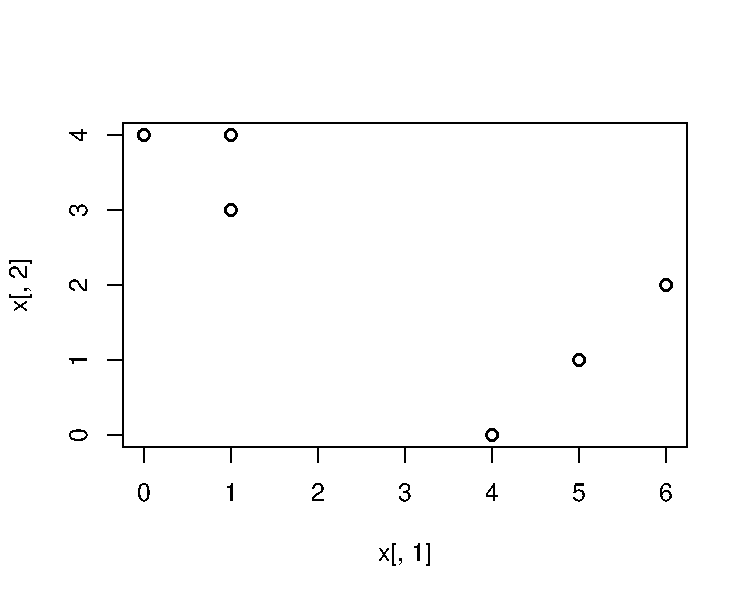
\includegraphics[width=\maxwidth]{figure/unnamed-chunk-2-1} 

}



\end{knitrout}
	
				\item \textit{Randomly assign a cluster label to each observation. You can use the sample() command in R to do this. Report the cluster labels for each observation.}		

\begin{knitrout}
\definecolor{shadecolor}{rgb}{0.969, 0.969, 0.969}\color{fgcolor}\begin{kframe}
\begin{alltt}
\hlstd{labs} \hlkwb{=} \hlkwd{sample}\hlstd{(}\hlnum{2}\hlstd{,} \hlkwd{nrow}\hlstd{(x),} \hlkwc{replace}\hlstd{=}\hlnum{TRUE}\hlstd{)}
\hlstd{labs}
\end{alltt}
\begin{verbatim}
## [1] 1 1 2 2 2 2
\end{verbatim}
\end{kframe}
\end{knitrout}
				
				\item \textit{Compute the centroid for each cluster.}
\begin{knitrout}
\definecolor{shadecolor}{rgb}{0.969, 0.969, 0.969}\color{fgcolor}\begin{kframe}
\begin{alltt}
\hlstd{cent1} \hlkwb{=} \hlkwd{c}\hlstd{(}\hlkwd{mean}\hlstd{(x[labs} \hlopt{==} \hlnum{1}\hlstd{,} \hlnum{1}\hlstd{]),} \hlkwd{mean}\hlstd{(x[labs} \hlopt{==} \hlnum{1}\hlstd{,} \hlnum{2}\hlstd{]))}
\hlstd{cent2} \hlkwb{=} \hlkwd{c}\hlstd{(}\hlkwd{mean}\hlstd{(x[labs} \hlopt{==} \hlnum{2}\hlstd{,} \hlnum{1}\hlstd{]),} \hlkwd{mean}\hlstd{(x[labs} \hlopt{==} \hlnum{2}\hlstd{,} \hlnum{2}\hlstd{]))}
\hlstd{cent1}
\end{alltt}
\begin{verbatim}
## [1] 1.0 3.5
\end{verbatim}
\begin{alltt}
\hlstd{cent2}
\end{alltt}
\begin{verbatim}
## [1] 3.75 1.75
\end{verbatim}
\end{kframe}
\end{knitrout}

				\item \textit{Assign each observation to the centroid to which it is closest, in terms of Euclidean distance. Report the cluster labels for each observation.}




\begin{knitrout}
\definecolor{shadecolor}{rgb}{0.969, 0.969, 0.969}\color{fgcolor}\begin{kframe}
\begin{alltt}
\hlcom{# in code have function that finds labs, echo set to F}
\hlstd{labs} \hlkwb{<-} \hlkwd{assign_labs}\hlstd{(x, cent1, cent2)}
\hlstd{labs}
\end{alltt}
\begin{verbatim}
## [1] 1 1 1 2 2 2
\end{verbatim}
\end{kframe}
\end{knitrout}
				
				\item \textit{In your plot from (a), color the observations according to the cluster labels obtained.}

\begin{knitrout}
\definecolor{shadecolor}{rgb}{0.969, 0.969, 0.969}\color{fgcolor}

{\centering 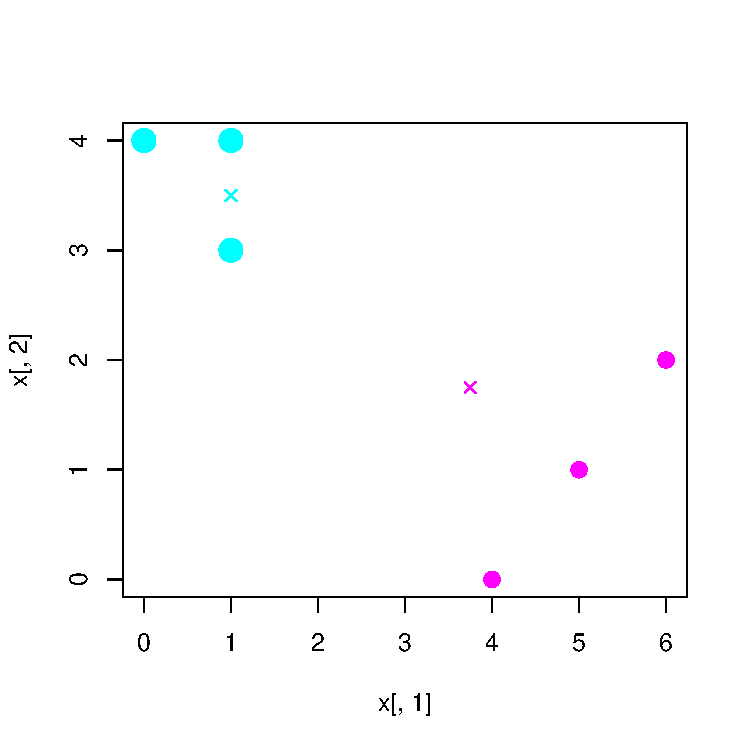
\includegraphics[width=\maxwidth]{figure/unnamed-chunk-7-1} 

}



\end{knitrout}

            
            \end{enumerate}



        \setcounter{enumi}{4}
		
		\item \textit{In words, describe the results that you would expect if you performed $K$-means clustering of the eight shoppers in Figure 10.14, on the basis of their sock and computer purchases, with $K = 2$. Give three answers, one for each of the variable scalings displayed. Explain.}
		
		\begin{enumerate}
			\item More computers and socks (1, 2, 7, 8) versus least socks and computer (3, 4, 6, 8).
			\item No computer (1, 2, 3, 4) versus a computer (5, 6, 7, 8). Distance is smaller on socks dimension whereas it is larger on the computer dimension. 
			
			\item (Similar to above) No computer (1, 2, 3, 4) against a computer (5, 6, 7, 8).
			
		\end{enumerate}
		
    \end{enumerate}



\end{document}

